\chapter{Introduzione}
Per l'esercizio assegnato si è voluto sperimentare l'effeto di vari parametri spesso oggetto di discussione nella preparazione di un buon caffè attraverso la moka.
Per questo si è fatta una ricerca sulle controversie tra cui le materie prime da utilizzare prima fra tutte l'acqua, la miscela di caffè che in questo esperimento sarà sempre la stessa.%
L'attenzione viene posta poi sulla prepaparazione ispezionando gli aspetti relativi alla quantità di acqua - o “sotto la volava" o “alla valova" - sulla quantità di caffè, ovvero filtro riempieti in maniera uniforme o formando la "montagnetta", l'operazine di pressatura o meno dela polvere prima della chiusura; infine la forza della fiamma se “alta" oppure “bassa”.
\begin{figure}[h]
  \centering
  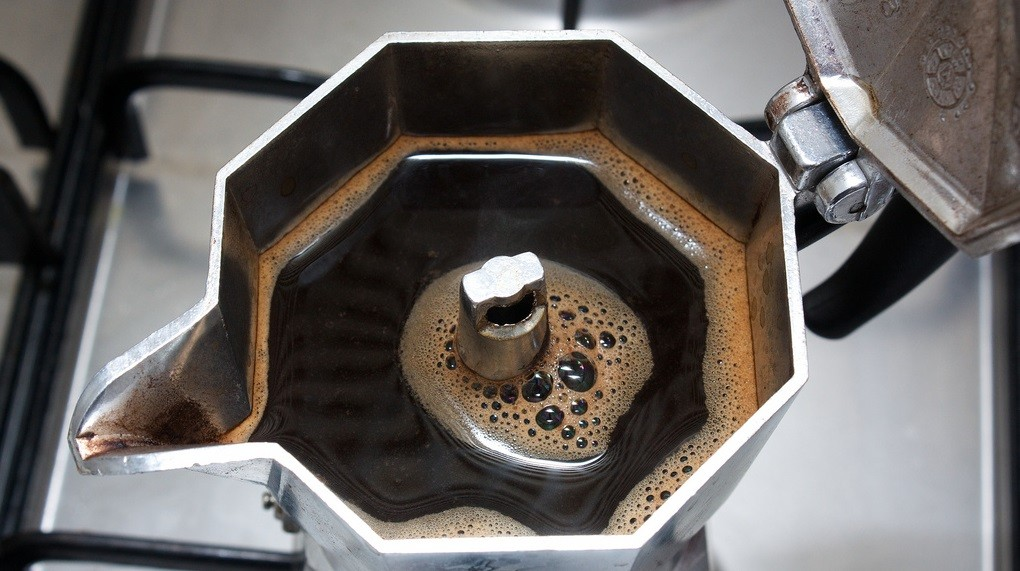
\includegraphics[width=0.80\textwidth]{2044770229}
  \caption{Caffè preparato con la moka}
  \label{fig:moka}
\end{figure}
\section{Materiali e strumenti}
\subsection{L'Acqua}
L' acqua scelte per la prova, che rappresenta buona parte del contenuto della tazza, è stata selezionata in base alle caratteristiche distiguendo secondo: la durezza e il residuo fisso.
\begin{itemize}
  \item Levissima (residuo fisso: 80,2 $mg/l$; durezza: 5,8 $^{\circ}$F, pH: 7,9)
  \item San Benedetto (residuo fisso: 268 $mg/l$, durezza: 21 $^{\circ}$F, pH: 7,5 )
\end{itemize}
La composizione dell’acqua, il rispettivo contenuto di ossigeno, così come il grado di durezza, le caratteristiche di equilibrio acido-base e il contenuto di minerali variano da sorgente a sorgente, da regione a regione. Questo è anche il motivo per il quale la cremosità del caffè e le caratteristiche di colore, aroma e gusto non sono mai le stesse.
In linea di principio vale la seguente regola: l’acqua con un maggior grado di durezza riduce l’aroma, l’acqua più dolce conferisce un gusto amaro.
Per conseguire i migliori risultati già in fase di preparazione del caffè occorre che l’acqua non sia né troppo dolce né troppo dura. L’acqua con un valore di durezza superiore neutralizza il leggero grado di acidità del caffè – con conseguente abbassamento del rispettivo grado di sapore. Più è lungo il tempo di contatto tra l'acqua e la polvere di caffè, più questo effetto è percettibile e di consequenza, il caffè perde aroma e sapore. D’altro canto anche l’acqua troppo dolce può compromettere il gusto del caffè\cite{mo_2017}\cite{acqua}.

\subsection{Moka e Caffè}
Per la prova si è optato per una caffettiera da tre tazze della Bialetti; contemporaneamente si è scelta la miscela di caffè Lavazza qualità "Rossa" di cui si riportano, dal sito del produttore\cite{Lavazza_2017}, le caratteristche:
\begin{itemize}
  \item Tostatura media: i cicli di tostatura di media lunghezza risaltano la fragranza e la dolcezza, soprattutto per le miscele di Arabica.
  \item Intesità: 5 -- caffè equilibrato e ricco di sapori.
\end{itemize}
\subsection{Strumenti di misura}
Si è utilizzata una bilancia elettronica da cuicna per misurare la massa di acqua e caffè durante la preparazione.
Per misurare i tempi di fuoriscita del caffè si è fatto di un iPhone 5 tramite l'applicazione del cronometro; le carattestiche sono riportate di seguito:
\begin{itemize}
  \item Bilancia elettronica da cucina “Krups"(portata max: 2000 [g], 0 - 1000: d = 2[g], 1000-2000: d = 5[g])
  \item iPhone 5 (iOS 10.3.3)
\end{itemize}

%=============================================================

\section{Preparazione}
Per ognuno dei fattori si sono scelti due livelli:
\begin{itemize}
  \item Livello dell'acqua: si associano due livelli quantitativi 130[g] e 160[g] di acqua che corrispondo ad una altezza d'acqua rispettivamnete inferiore alla valvola e all'altezza della valvola.
  \item Tipo di acqua: si associa un fattore di qualità d'acqua per quanto riguardano le loro caratteristiche intrisiche;
  \item Quantità di caffè: si assci un fattore quantitativo espresso in peso, anche qui si è scelto di valutare una quantità di caffè che riempie il filtro in maniera omogenea pari a 18[g] ed un livello superiore dove s va formare la “montagnetta" fissata ad un peso di 22 [g].
  \item Pressatura: è intesa come fattore qualitativo in quanto condizione del caffè all'interno del filtro prima della chiusura della parte superiore.
  \item Fiamma: fattore qualitativo che presenta due stati la posizione della manopola in posizione di alta e bassa ripsettivamente.
\end{itemize}
In tabella \ref{tab:factorLvl} si riporta in forma sintetica i valori e livelli dei fattori prima descritti associando ad essi gli identificativi convenzionali.

\begin{table}[htb]
  \caption{Fattori e livelli}
  \label{tab:factorLvl}
  \begin{tabular}{cccccc}
    \hline
    & Quantità di acqua & Tipo acqua & Quantita di caffè & Pressatura & Fiamma\\
    & [g] &  & [g] &  & \\
    \hline
    & A &B&C&D&E\\
    \hline
  + & 160 & San Benedetto & 24 & Si & Alta\\
  - & 130 & Levissima & 18 & No & Bassa\\
  \hline
  \end{tabular}
\end{table}
\newpage
\section{L'esperimento}
Seguendo l'esempio delle lezioni si è realizzata una funzione per generare la design matrix  e la salva su un file per poi completarla e successivamente una volta esegute le prove.
All'interno della funzione si è fatto uso della funzione \emph{gl()} per generare sequenze ordinate di fattori e la gnerazione di una chiave di ordinazione casuale.
Le prove sono state eseguite seguendo il \emph{RunOrder} riportato nella design matrix in quanto sono state eseguite più prove nello stesso giorno.
La base della caffettiera è stata riempita con acqua fredda secondo i livelli prima descritti, pesando di volta in volta la quantità di acqua nella caldaia. Succesivamente si prosegue con la deposizione del caffe nel filtro in quantità prescritte dalla prova ed effettuta una pressatura o meno. Viene avvitata la parte superiore della caffetiera e posizionata sul fornello piu piccolo del piano cottura regolandone la fiamma conteporanemante si avvia il cronometro.
L'alimentazione viene spenta quando il caffè è risalito completamente, si ferma il cronometro, viene pesata la quantità di caffè fuoriscita sulla bialanica ed infine si registra iniseme al tempo.
